\chapter{Software Requirements Specifications} \label{ch
}

This chapter outlines the detailed functional and non-functional requirements for the project. It includes descriptions of the main features, quality attributes, and system specifications to guide the development process.

\section{List of Features} The primary features of the project include: \begin{itemize} \item Real-time posture and facial expression analysis using AI. \item Interactive interview simulation with dynamic question selection. \item Detailed feedback and analysis report on user performance. \item User account management, including login, signup, and profile settings. \item Integration with webcam for real-time feedback. \end{itemize}

\section{Functional Requirements} The functional requirements detail the specific functions and capabilities of the system: \begin{itemize} \item The system shall allow users to log in, sign up, and manage their profiles. \item The system shall analyze users' facial expressions and posture through the webcam. \item The system shall present users with interview questions and evaluate their responses. \item The system shall generate a feedback report, highlighting performance and improvement areas. \item The system shall support both manual and Google login options. \end{itemize}

\section{Quality Attributes} Quality attributes are non-functional characteristics that are crucial for system success: \begin{itemize} \item Usability: The system should provide an intuitive and easy-to-use interface. \item Reliability: The feedback provided by the AI should be accurate and dependable. \item Performance: The system should perform real-time analysis without noticeable delays. \item Scalability: The platform should handle a high number of users with minimal performance degradation. \item Security: All user data, including video data, must be securely handled and stored. \end{itemize}

\section{Non-Functional Requirements} Non-functional requirements define system characteristics: \begin{itemize} \item Performance Requirements: The analysis of user performance should complete within 2 seconds of response. \item Security Requirements: User data should be encrypted and securely stored. \item Accessibility: The application should be accessible to people with different levels of computer proficiency. \item Compatibility: The application should be compatible with standard webcam devices and browsers. \end{itemize}

\section{Use Cases/ Use Case Diagram} The use case diagram in Figure~\ref{fig
} below illustrates the system’s interactions with different types of users. It highlights how various actors engage with key system functionalities, providing a high-level view of user roles and their access to features.

\begin{figure}[h] \centering 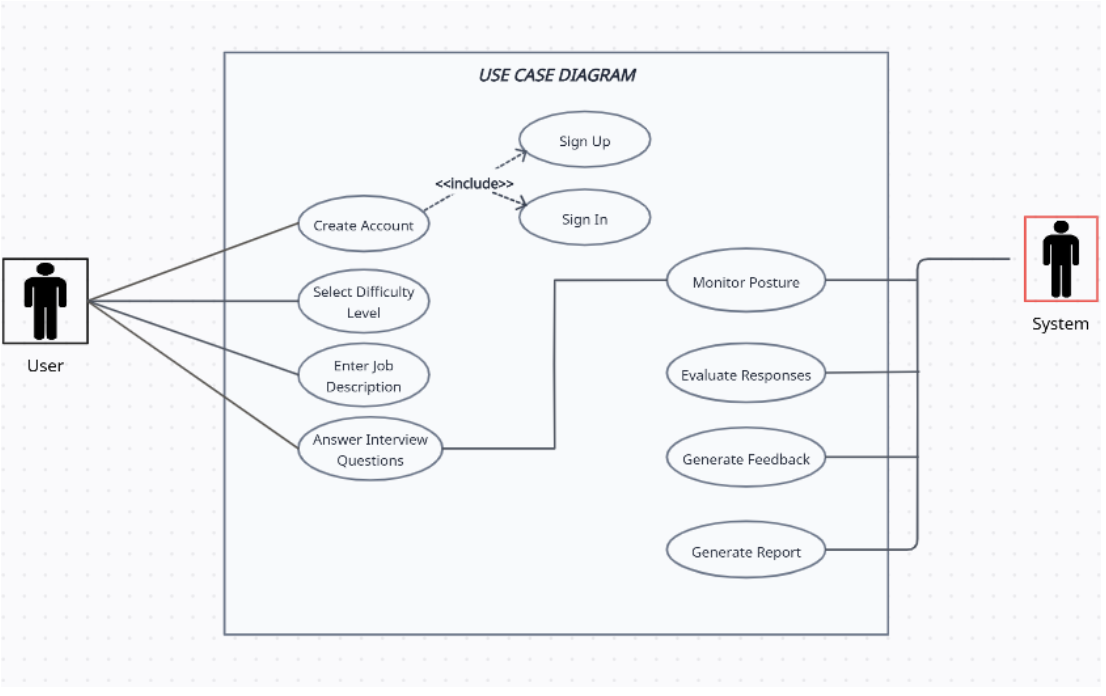
\includegraphics[width=0.5\linewidth]{sections/diagrams/UseCase.png} \caption{Use Case Diagram of the System} \label{fig
} \end{figure}

\section{Sequence Diagrams/System Sequence Diagram} This section includes sequence diagrams that illustrate the order of interactions within the system. These diagrams depict the step-by-step processes for key functionalities, such as user login, interview simulation, and report generation. They provide a clear visualization of how users interact with the system and how various components communicate to execute tasks efficiently.

\begin{figure}[h] \centering 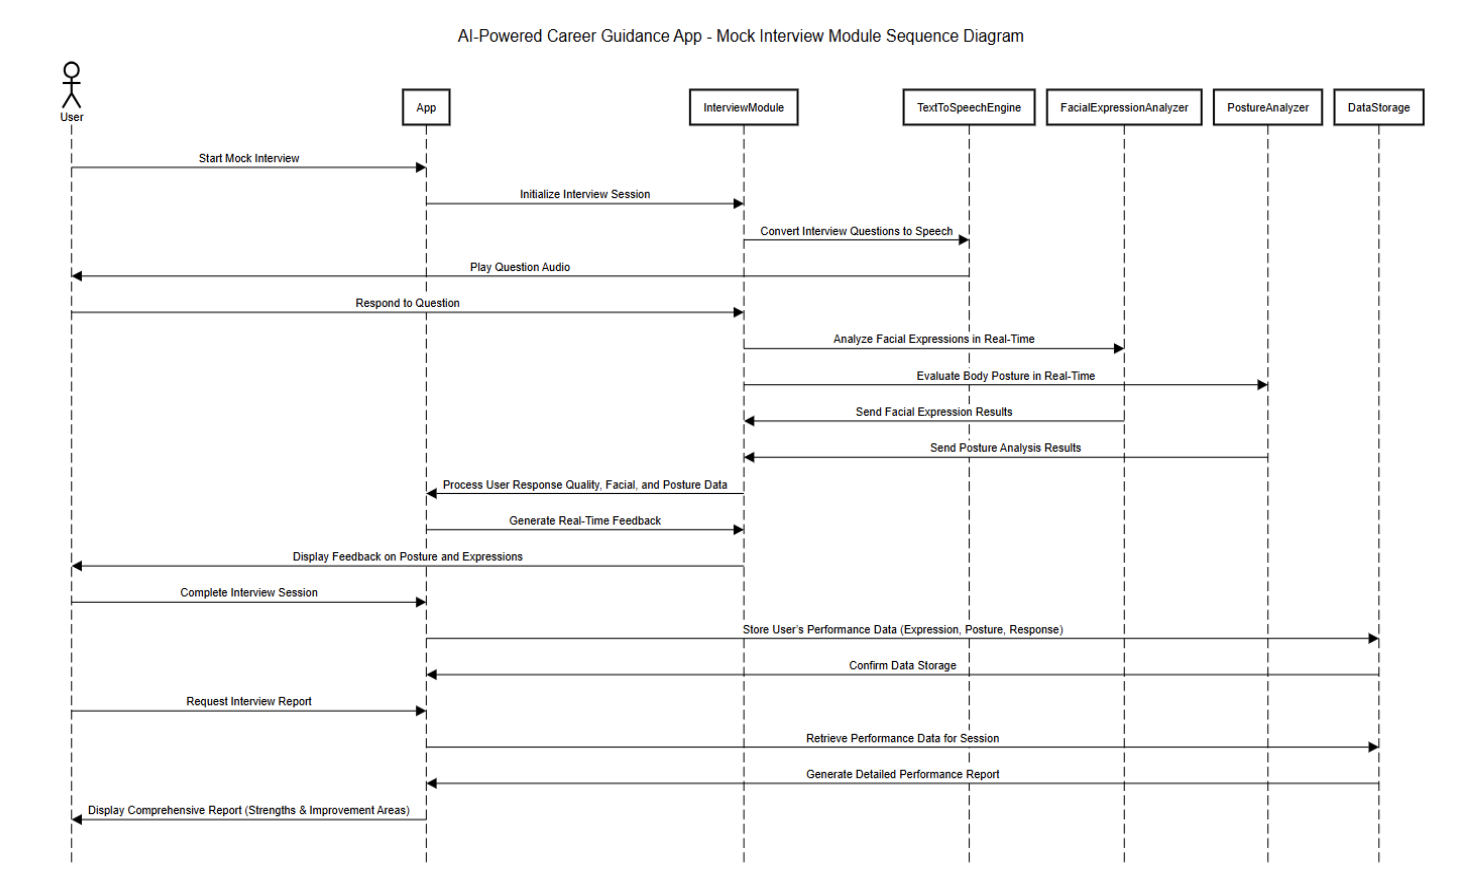
\includegraphics[width=0.5\linewidth]{sections/diagrams/SequentialModel.png} \caption{Sequence Diagram of Key Functionalities} \label{fig
} \end{figure}

\section{Architecture Diagram} This section includes an architecture diagram that illustrates the overall structure of the system. The diagram provides a high-level view of the system's components and their interactions, highlighting how different modules communicate with each other. Key functionalities such as user login, interview simulation, and report generation are represented, showcasing the integration of various technologies and frameworks that support the application’s operation.

\begin{figure}[h] \centering 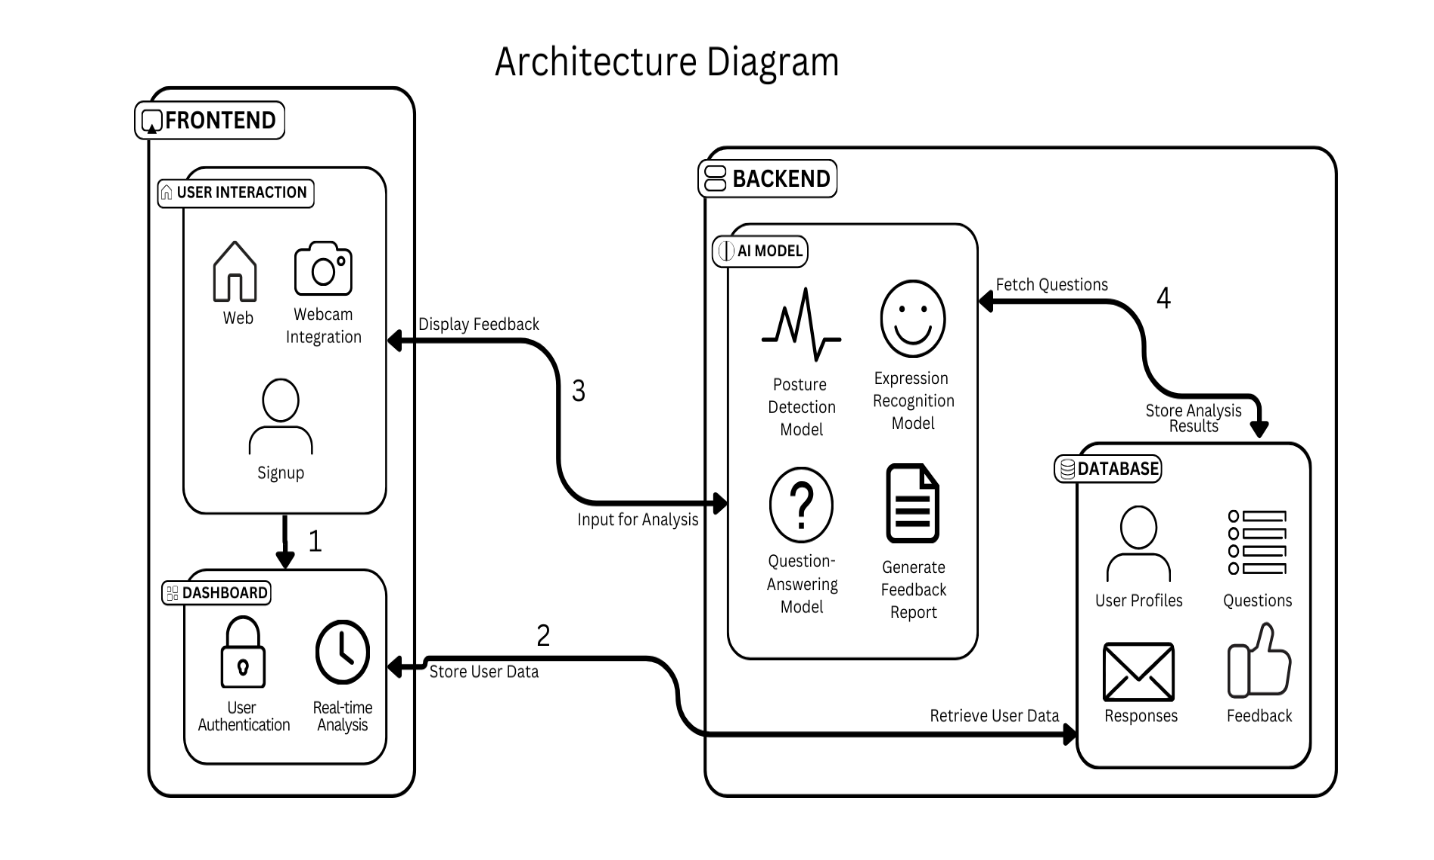
\includegraphics[width=0.5\linewidth]{sections/diagrams/ArchitectureDiagram.png} \caption{Architecture Diagram of the System} \label{fig
} \end{figure}

\section{Test Plan (Test Level, Testing Techniques)} The test plan will outline the levels of testing, including: \begin{itemize} \item Unit Testing: Testing individual components, such as user authentication and report generation. \item Integration Testing: Ensuring all system components work together, including the AI analysis and report generation. \item System Testing: Testing the complete system functionality and performance under various conditions. \item User Acceptance Testing (UAT): Ensuring the final product meets user expectations and requirements. \end{itemize}

Testing techniques will include both manual and automated testing.

\section{Software Development Plan} The software development plan will detail the project timeline, development methodology (e.g., Agile), key milestones, and resource allocation. Development phases will cover requirements gathering, design, implementation, testing, and deployment.

\section{Wire-frames} This section will include wireframes of the major screens in the application, such as the login page, interview simulation screen, and feedback report page. Wireframes provide a visual blueprint for the user interface and layout.

\section{UI Screens} The UI screens will include final designs of the user interface, showcasing elements like buttons, navigation, and layout for a consistent user experience. These will be developed based on the wireframes and refined to ensure usability and visual appeal.